\documentclass[11pt,a4j,uplatex]{jsarticle}
\usepackage{ascmac}
\usepackage{amsmath}
\usepackage[dvipdfmx]{graphicx}
\usepackage{upgreek}

\newsavebox{\circlebox}
\savebox{\circlebox}{\fontencoding{OMS}\selectfont\Large\char13}
\newlength{\circleboxwdht}
\newcommand{\centercircle}[1]{%
  \setlength{\circleboxwdht}{\wd\circlebox}%
  \addtolength{\circleboxwdht}{\dp\circlebox}%
  \raisebox{0.4\dp\circlebox}{%
    \parbox[][\circleboxwdht][c]{\wd\circlebox}{\centering#1}}%
  \llap{\usebox{\circlebox}}%
}	%丸数字(文字)環境。\centercircle{入れたい文字} で丸文字を表示する。


\title{宮島研究室2019年度B4スタート実験}
\author{東京理科大学 応用物理学科 宮島研究室B4 渡辺慧}
\date{\today}


\begin{document}

\maketitle %タイトル

\thispagestyle{empty}%このページにはページ番号を入れない.
\clearpage
\addtocounter{page}{-1}

\newpage

\tableofcontents %目次

\thispagestyle{empty}%このページにはページ番号を入れない
\clearpage
\addtocounter{page}{-1}

\listoffigures%図目次。確認用。後で消す

\newpage
\section{本研究の目的}
本研究の目的は、物質の光学反応を観測する際に用いる分光計を正しく取り扱い、CdS、GaAs及びGaAs/AlGaAs多重量子井戸の発光の特性を測定することである。

\section{原理}
\subsection{NaCl粉末の回折パターン}

\begin{table}[htbp]
 \begin{center}
  \caption{NaCl粉末の回折パターン\cite{powder}}
  \begin{tabular}{|l|l|l|l|l|l|}  \hline
           & \multicolumn{3}{l}{Miller Indices} &   &                                \\
   $2\theta(°)$  & h                                  & k & l & Intensity & d-spacing [nm] \\  \hline \hline
   26.886  & 1                                  & 1 & 1 & 10        & 0.3312         \\
   31.145  & 2                                  & 0 & 0 & 99        & 0.2869         \\
   44.629  & 2                                  & 2 & 0 & 61        & 0.2028         \\
   52.878  & 3                                  & 1 & 1 & 3         & 0.173          \\
   55.426  & 2                                  & 2 & 2 & 19        & 0.1656         \\
   64.959  & 4                                  & 0 & 0 & 8         & 0.1434         \\
   71.633  & 3                                  & 3 & 1 & 2         & 0.1316         \\
   73.797  & 4                                  & 2 & 0 & 19        & 0.1283         \\
   82.251  & 4                                  & 2 & 2 & 13        & 0.1171         \\
   88.472  & 5                                  & 1 & 1 & 2         & 0.1104         \\
   98.837  & 4                                  & 4 & 0 & 4         & 0.1014         \\
   105.176 & 5                                  & 3 & 1 & 2         & 0.097          \\
   107.328 & 6                                  & 0 & 0 & 8         & 0.0956         \\
   107.328 & 4                                  & 4 & 2 & 8         & 0.0956         \\
   116.236 & 6                                  & 2 & 0 & 6         & 0.0907         \\
   125.896 & 6                                  & 2 & 2 & 5         & 0.0865         \\
   136.933 & 4                                  & 4 & 4 & 2         & 0.0828         \\
   147.009 & 7                                  & 1 & 1 & 2         & 0.0803         \\
   147.009 & 5                                  & 5 & 1 & 2         & 0.0803         \\
   151.023 & 6                                  & 4 & 0 & 4         & 0.0796         \\  \hline
  \end{tabular}
  \label{***label***}
 \end{center}
\end{table}


\newpage
\section{NaCl粉末及び単結晶の回折パターンの解析}


\subsection{NaCl粉末}

NaCl粉末における回折パターンを図\ref{powder}に示す。

\begin{figure}[htb]
 \centering
 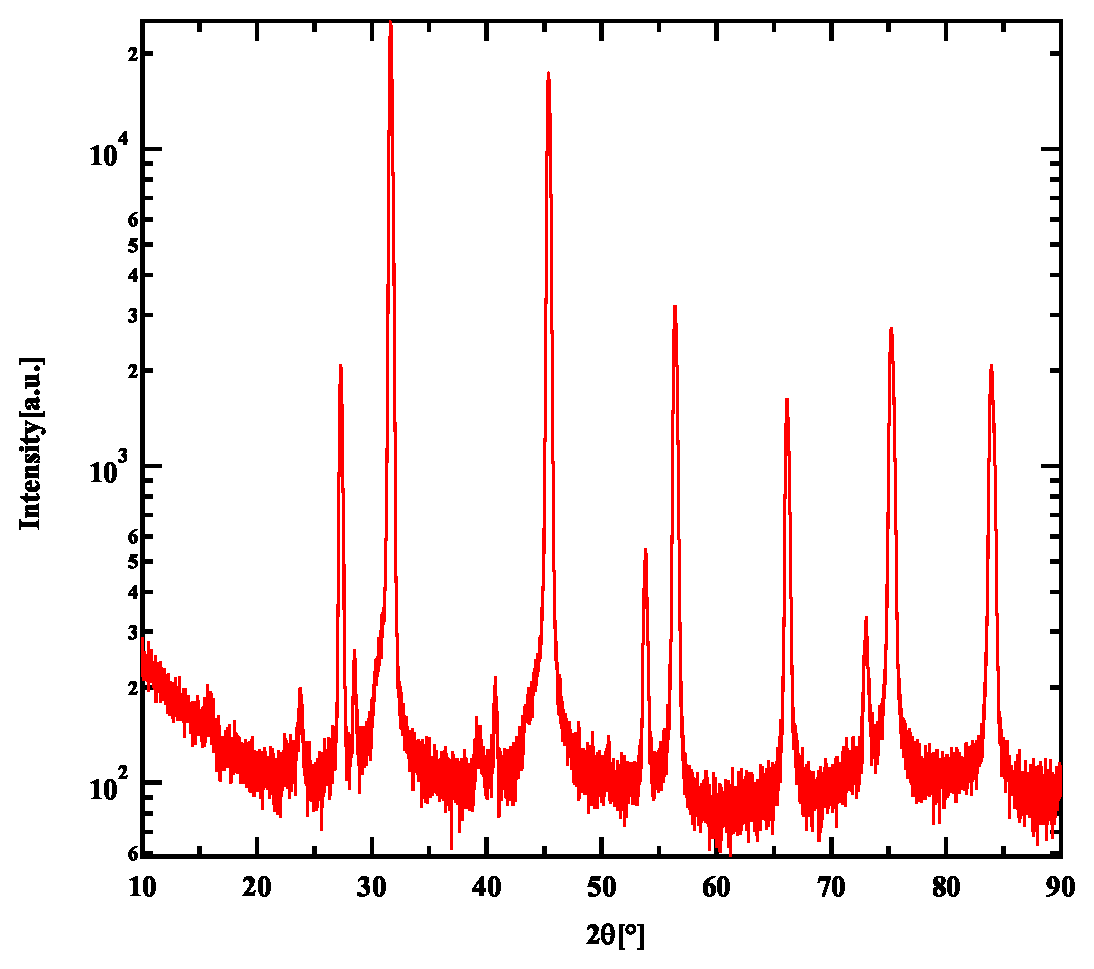
\includegraphics[clip,width=9cm]{FigPowder.eps}
 \caption{NaCl粉末の回折パターン.}
 \label{powder}
\end{figure}



\subsection{NaCl単結晶}

図\ref{bulk}に示す。

\begin{figure}[htb]
 \centering
 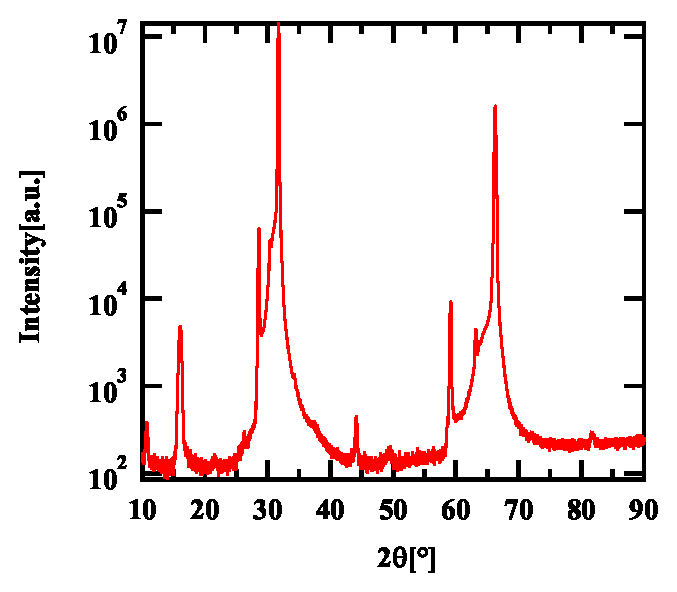
\includegraphics[clip,width=9cm]{FigBulk.eps}
 \caption{NaCl結晶の回折パターン.}
 \label{bulk}
\end{figure}


\newpage
%参考文献。\cite{タグ}で参照を示せる。
\begin{thebibliography}{9}
 \bibitem{powder}株式会社島津 https://www.shimadzu.co.jp/products/opt/guide/07.html 2019/4/12
 \bibitem{CCD} キヤノンサイエンスラボ https://global.canon/ja/technology/s\_labo/light/003/04.html 2019/04/12
 \bibitem{Fibor} 分光計器株式会社 http://www.bunkoukeiki.co.jp/technology.fiber.html 2019/04/12
 \bibitem{varshni}Y.P.Varshni TEMPERATURE DEPENDENCE OF THE ENERGY GAP IN SEMICONDUCTORS
 \bibitem{gapE}キッテル固体物理学入門上第8版 p.119


\end{thebibliography}

\end{document}
